\documentclass[]{report}
\usepackage[table,xcdraw]{xcolor}
\usepackage[Glenn]{fncychap}
\usepackage[T1]{fontenc}
\usepackage[francais]{babel}
\usepackage{wrapfig}
\usepackage{graphicx}
\usepackage[a4paper, width=185mm, top=15mm, bottom=15mm]{geometry}
\usepackage{parskip}
\usepackage{enumitem}
\usepackage{titlesec}
\usepackage{listings}
\usepackage{float}
\usepackage[final]{pdfpages}
\usepackage{tocbibind}
\usepackage{tocloft}
\usepackage{xpatch}
\usepackage{amsmath}
\usepackage{amsthm}
\usepackage{amsfonts}
\usepackage{graphics}
\usepackage{framed}
\usepackage{multirow}
\usepackage{graphicx}
\usepackage[utf8x]{inputenc}
\usepackage{mathtools}
\usepackage{amsmath}
\usepackage{tabularx}
\usepackage{tikz}
\usepackage{multirow}
\usepackage[noend]{algpseudocode}
\usepackage{tabularx}  % for tabularx
\usepackage{arabtex}
\usepackage{utf8}
\usepackage{hyperref}
\hypersetup{
	colorlinks = true,
	linkbordercolor = {white},
	linkcolor=blue
}

\usepackage{listings}
\usepackage{color}

\definecolor{dkgreen}{rgb}{0,0.6,0}
\definecolor{gray}{rgb}{0.5,0.5,0.5}
\definecolor{mauve}{rgb}{0.58,0,0.82}
\definecolor{gray}{rgb}{0.4,0.4,0.4}
\definecolor{darkblue}{rgb}{0.0,0.0,0.6}
\definecolor{lightblue}{rgb}{0.0,0.0,0.9}
\definecolor{cyan}{rgb}{0.0,0.6,0.6}
\definecolor{darkred}{rgb}{0.6,0.0,0.0}

\definecolor{maroon}{cmyk}{0, 0.87, 0.68, 0.32}
\definecolor{halfgray}{gray}{0.55}
\definecolor{ipython_frame}{RGB}{207, 207, 207}
\definecolor{ipython_bg}{RGB}{247, 247, 247}
\definecolor{ipython_red}{RGB}{186, 33, 33}
\definecolor{ipython_green}{RGB}{0, 128, 0}
\definecolor{ipython_cyan}{RGB}{64, 128, 128}
\definecolor{ipython_purple}{RGB}{170, 34, 255}

\lstset{
	escapeinside=``,
	basicstyle=\ttfamily\footnotesize,
	columns=fullflexible,
	showstringspaces=false,
	numbers=left,                   % where to put the line-numbers
	numberstyle=\tiny\color{gray},  % the style that is used for the line-numbers
	stepnumber=1,
	numbersep=5pt,                  % how far the line-numbers are from the code
	backgroundcolor=\color{white},      % choose the background color. You must add \usepackage{color}
	showspaces=false,               % show spaces adding particular underscores
	showstringspaces=false,         % underline spaces within strings
	showtabs=false,                 % show tabs within strings adding particular underscores
	frame=none,                   % adds a frame around the code
	rulecolor=\color{black},        % if not set, the frame-color may be changed on line-breaks within not-black text (e.g. commens (green here))
	tabsize=2,                      % sets default tabsize to 2 spaces
	captionpos=b,                   % sets the caption-position to bottom
	breaklines=true,                % sets automatic line breaking
	breakatwhitespace=false,        % sets if automatic breaks should only happen at whitespace
	title=\lstname,                   % show the filename of files included with \lstinputlisting;
	% also try caption instead of title  
	commentstyle=\color{gray}\upshape
}


\lstdefinelanguage{XML}
{
	morestring=[s][\color{mauve}]{"}{"},
	morestring=[s][\color{black}]{>}{<},
	morecomment=[s]{<?}{?>},
	morecomment=[s][\color{dkgreen}]{<!--}{-->},
	stringstyle=\color{black},
	identifierstyle=\color{lightblue},
	keywordstyle=\color{red},
	morekeywords={xmlns,xsi,noNamespaceSchemaLocation,type,id,x,y,source,target,version,tool,transRef,roleRef,objective,eventually}% list your attributes here
}

\usepackage{bera}% optional: just to have a nice mono-spaced font
\usepackage{xcolor}

\colorlet{punct}{red!60!black}
\definecolor{background}{HTML}{EEEEEE}
\definecolor{delim}{RGB}{20,105,176}
\colorlet{numb}{magenta!60!black}

\lstdefinelanguage{json}{
	basicstyle=\normalfont\ttfamily,
	numbers=left,
	numberstyle=\scriptsize,
	stepnumber=1,
	numbersep=8pt,
	showstringspaces=false,
	breaklines=true,
	frame=lines,
	literate=
	*{0}{{{\color{numb}0}}}{1}
	{1}{{{\color{numb}1}}}{1}
	{2}{{{\color{numb}2}}}{1}
	{3}{{{\color{numb}3}}}{1}
	{4}{{{\color{numb}4}}}{1}
	{5}{{{\color{numb}5}}}{1}
	{6}{{{\color{numb}6}}}{1}
	{7}{{{\color{numb}7}}}{1}
	{8}{{{\color{numb}8}}}{1}
	{9}{{{\color{numb}9}}}{1}
	{:}{{{\color{punct}{:}}}}{1}
	{,}{{{\color{punct}{,}}}}{1}
	{\{}{{{\color{delim}{\{}}}}{1}
	{\}}{{{\color{delim}{\}}}}}{1}
	{[}{{{\color{delim}{[}}}}{1}
	{]}{{{\color{delim}{]}}}}{1},
}


\lstdefinelanguage{python}{
	morekeywords={access,and,break,class,continue,def,del,elif,else,except,exec,finally,for,from,global,if,import,in,is,lambda,not,or,pass,print,raise,return,try,while},
	morekeywords=[2]{abs,all,any,basestring,bin,bool,bytearray,callable,chr,classmethod,cmp,compile,complex,delattr,dict,dir,divmod,enumerate,eval,execfile,file,filter,float,format,frozenset,getattr,globals,hasattr,hash,help,hex,id,input,int,isinstance,issubclass,iter,len,list,locals,long,map,max,memoryview,min,next,object,oct,open,ord,pow,property,range,raw_input,reduce,reload,repr,reversed,round,set,setattr,slice,sorted,staticmethod,str,sum,super,tuple,type,unichr,unicode,vars,xrange,zip,apply,buffer,coerce,intern},
	sensitive=true,
	morecomment=[l]\#,
	morestring=[b]',
	morestring=[b]",
	morestring=[s]{'''}{'''},
	morestring=[s]{"""}{"""},
	morestring=[s]{r'}{'},
	morestring=[s]{r"}{"},
	morestring=[s]{r'''}{'''},
	morestring=[s]{r"""}{"""},
	morestring=[s]{u'}{'},
	morestring=[s]{u"}{"},
	morestring=[s]{u'''}{'''},
	morestring=[s]{u"""}{"""},
	% {replace}{replacement}{lenght of replace}
	% *{-}{-}{1} will not replace in comments and so on
	literate=
	{á}{{\'a}}1 {é}{{\'e}}1 {í}{{\'i}}1 {ó}{{\'o}}1 {ú}{{\'u}}1
	{Á}{{\'A}}1 {É}{{\'E}}1 {Í}{{\'I}}1 {Ó}{{\'O}}1 {Ú}{{\'U}}1
	{à}{{\`a}}1 {è}{{\`e}}1 {ì}{{\`i}}1 {ò}{{\`o}}1 {ù}{{\`u}}1
	{À}{{\`A}}1 {È}{{\'E}}1 {Ì}{{\`I}}1 {Ò}{{\`O}}1 {Ù}{{\`U}}1
	{ä}{{\"a}}1 {ë}{{\"e}}1 {ï}{{\"i}}1 {ö}{{\"o}}1 {ü}{{\"u}}1
	{Ä}{{\"A}}1 {Ë}{{\"E}}1 {Ï}{{\"I}}1 {Ö}{{\"O}}1 {Ü}{{\"U}}1
	{â}{{\^a}}1 {ê}{{\^e}}1 {î}{{\^i}}1 {ô}{{\^o}}1 {û}{{\^u}}1
	{Â}{{\^A}}1 {Ê}{{\^E}}1 {Î}{{\^I}}1 {Ô}{{\^O}}1 {Û}{{\^U}}1
	{œ}{{\oe}}1 {Œ}{{\OE}}1 {æ}{{\ae}}1 {Æ}{{\AE}}1 {ß}{{\ss}}1
	{ç}{{\c c}}1 {Ç}{{\c C}}1 {ø}{{\o}}1 {å}{{\r a}}1 {Å}{{\r A}}1
	{€}{{\EUR}}1 {£}{{\pounds}}1
	%
	{^}{{{\color{ipython_purple}\^{}}}}1
	{=}{{{\color{ipython_purple}=}}}1
	%
	{+}{{{\color{ipython_purple}+}}}1
	{*}{{{\color{ipython_purple}$^\ast$}}}1
	{/}{{{\color{ipython_purple}/}}}1
	%
	{+=}{{{+=}}}1
	{-=}{{{-=}}}1
	{*=}{{{$^\ast$=}}}1
	{/=}{{{/=}}}1,
	literate=
	*{-}{{{\color{ipython_purple}-}}}1
	{?}{{{\color{ipython_purple}?}}}1,
	%
	identifierstyle=\color{black}\ttfamily,
	commentstyle=\color{ipython_cyan}\ttfamily,
	stringstyle=\color{ipython_red}\ttfamily,
	keepspaces=true,
	showspaces=false,
	showstringspaces=false,
	rulecolor=\color{ipython_frame},
	frame=single,
	frameround={t}{t}{t}{t},
	framexleftmargin=6mm,
	numbers=left,
	numberstyle=\tiny\color{halfgray},
	% extendedchars=true,
	basicstyle=\scriptsize,
	keywordstyle=\color{ipython_green}\ttfamily,
}


%\lstset{
%	literate=%
%	{à}{{\'a}}1
%	{í}{{\'i}}1
%	{é}{{\'e}}1
%	{è}{{\`e}}1
%	{ý}{{\'y}}1
%	{ú}{{\'u}}1
%	{ó}{{\'o}}1
%	{ě}{{\v{e}}}1
%	{š}{{\v{s}}}1
%	{č}{{\v{c}}}1
%	{ř}{{\v{r}}}1
%	{ž}{{\v{z}}}1
%	{ď}{{\v{d}}}1
%	{ť}{{\v{t}}}1
%	{ň}{{\v{n}}}1
%	{ů}{{\r{u}}}1
%	{Á}{{\'A}}1
%	{Í}{{\'I}}1
%	{É}{{\'E}}1
%	{Ý}{{\'Y}}1
%	{Ú}{{\'U}}1
%	{Ó}{{\'O}}1
%	{Ě}{{\v{E}}}1
%	{Š}{{\v{S}}}1
%	{Č}{{\v{C}}}1
%	{Ř}{{\v{R}}}1
%	{Ž}{{\v{Z}}}1
%	{Ď}{{\v{D}}}1
%	{Ť}{{\v{T}}}1
%	{Ň}{{\v{N}}}1
%	{Ů}{{\r{U}}}1
%}

\begin{document}

\setcode{utf8}


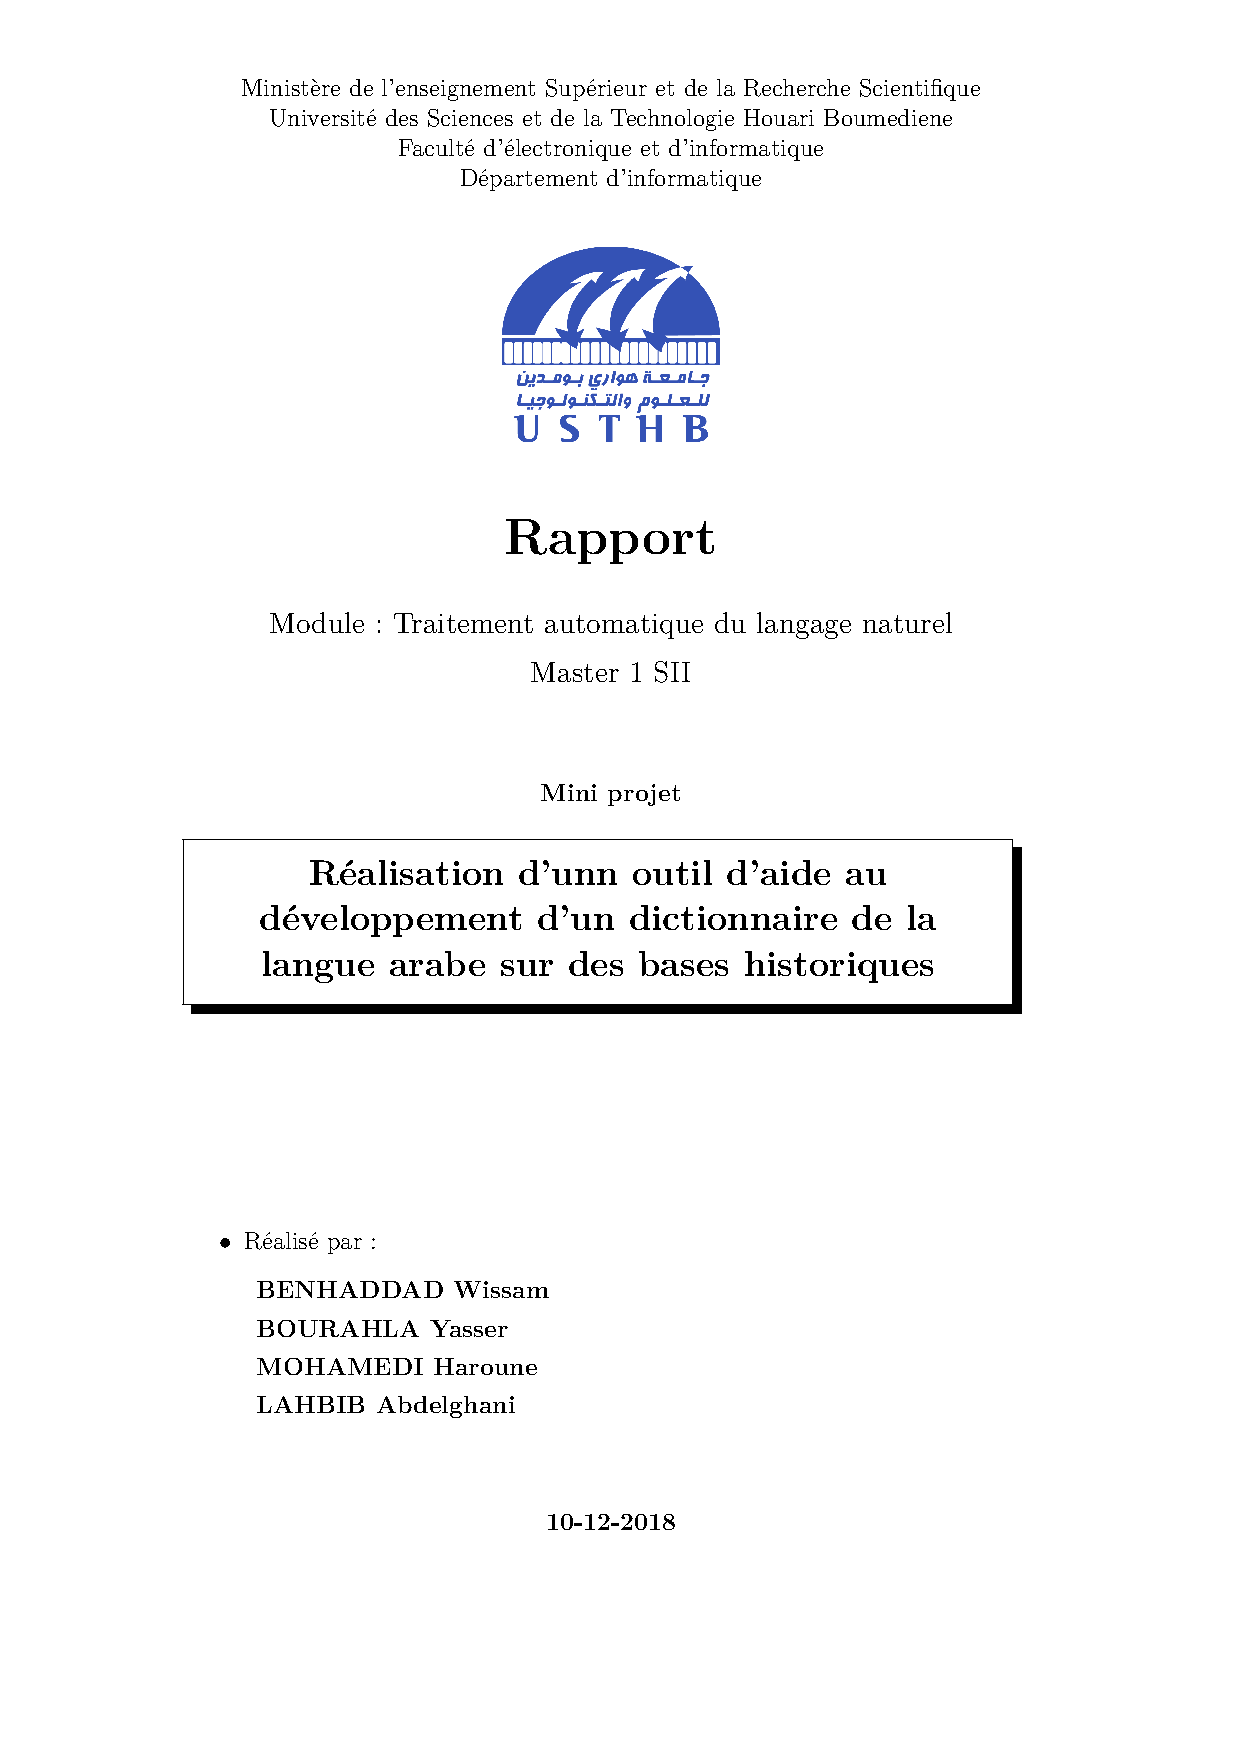
\includepdf[pages=1]{Page_garde.pdf} 

\tableofcontents

\listoffigures
	
\chapter{Motivations et problématique}
	\section{Introduction}
		\paragraph{}
		Depuis son apparition (au IIe siècle), la langue arabe n'a cessé d'évoluer, donnant naissance à de nouveaux mots, ou modifiant le sens de mots existants. Cette évolution a particulièrement enrichi le vocabulaire de la langue de l'islam, en conséquent et au fil du temps, plusieurs ouvrages destiné a recenser les différentes définitions et sens d'un mot ont vu le jour, chacun durant sa période. néanmoins,  il est primordial de garder une trace des différents changement qui ont eu lieu sur ces mots, et cela depuis leurs émergence. C'est avec cette idée en tête que les lexicographes des temps modernes en eu l'initiative d'entamer la construction de dictionnaires historiques afin de regrouper toutes les nuances des mots a travers les ages.
		\par
		La création d'un tel ouvrage n'est pas chose facile, en effet elle demande d'une part une grande connaissance sur les différentes périodes historiques de la langue, ainsi que sur la langue en elle même durant ces périodes. Chercher et regrouper des écrits, documents et ouvrages des différentes auteurs durant ces périodes est une tâche qui est en elle même très ardue, cela peut prendre plusieurs décennies pour créer une collection de documents asses représentative de chaque période. Analyser le contenue de tout ces documents est la phase qui dure le plus de temps, une vérification minutieuse de chaque information ajoutée au dictionnaire finale doit être faite, puis sujette à l'approbation de plusieurs experts du domaine.
		\par
		C'est avec l'avènement de l'informatique, de l'intelligence artificielle et plus récemment avec l'explosion du volume de données présent sur internet, que l'idée d'utiliser ces technologies pour faciliter et accélérer le processus de création d'un dictionnaire historique de la langue arabe à émergé. En effet la grande quantité et diversité de documents présente sur internet pourrait être exploité par un lexicographe pour ne pas s'attarder sur fastidieuse tâche de collecte des données, et cela en utilisant des techniques de traitement automatique du langage (TALN), de recherche d'information(RI) et d'intelligence artificielle.
		\par
		Ce besoin d'un outillage informatique est la principale motivation derrière ce mini-projet, avec suffisamment de données et une bonne conception, la réalisation d'un tel outillage pourrait faire gagner énormément de temps aux lexicographes du monde arabe.
		\par 
		Le but de projet étant maintenant établi, nous allons maintenant passer à la schématisation de ce rapport. Nous commencerons d'abord par de petites définitions pour se situer dans la suite du rapport, nous enchaînerons ensuite sur la conception du système pour expliquer le travail réalisé, viendra ensuite la présentation de notre application, enfin nous finirons par une conclusion générale comportant un bilan du projet, des critiques sur notre système ainsi que les perspectives envisagées.
	\newpage
	\section{Définitions}
		\subsection{DataSet et Corpus}
		\paragraph{}
		Un jeu de données (DataSet) est un ensemble de données traité et organisé dans un schéma spécifique aux besoins d'un système, un dataset peut être une base de données relationnelle, un ensemble de fichiers texte, une banque d'images/videos ...
		\par Dans notre cas nous nous intéresserons plus particulièrement à un type de dataset appelé Corpus, informellement un corpus est un dataset principalement utilisé dans le domaine du TALN, il est constitué d'un ensemble de fichier texte (annotés ou pas) qui représentent un domaine, une thématique, un(ou des) type(s) d'ouvrages ...
		\par Un corpus est un composant essentiel pour la l'application des techniques de TALN, la taille et la qualité d'un corpus est donc un facteur primordial pour assurer une bonne performance d'un système.
		\subsection{TALN}
			\paragraph{}
			Le Traitement Automatique du Langage Naturel (TALN) est un sous domaine de l'intelligence artificielle qui vise à analyser et à modéliser les composants du langage humain, que ce soit du point de vue syntaxique, sémantique ou pragmatique. l'aspect principal du TALN est le fait de permettre aux machine de traiter les séquence de texte non plus comme une simple suite de symboles, mais comme des entités informationnelles. Des connaissances sur la langue sont un prérequis essentiel pour le développement d'un système utilisant le TALN, ainsi que la disponibilité d'un grand ensemble de données pour faire de l'apprentissage automatique.
			\par 
			Le TALN est découpé en un ensemble de techniques et opérations à appliquer sur du texte, une multitude de domaine d'application existent pour l'utilisation de ces derniers. Dans ce projet nous nous intéresserons principalement aux techniques suivantes :  
			\subsubsection{Lemmatisation} 
				\paragraph{}
				La lemmatisation est un terme désignant l’analyse lexicale d’un texte dans le but de regrouper les mots d’une même famille. Les mots d’une même famille sont donc réduits en une unique entité appelée « \textbf{lemme} ».
				Ainsi la lemmatisation consiste à regrouper les différentes flexions d’un mot unique.\cite{lemme}
				
			\subsubsection{Segmentation}
				\paragraph{}
				La segmentation d'un texte est l'opération de découpage de ce dernier en composantes linguistiques plus petites(des phrases, des groupes nominaux, des mots ...), c'est un processus non-trivial car chaque langue dispose de règles spécifiques en ce qui concerne les marqueurs de fin de phrases.
			
			\subsubsection{Étiquetage morphosyntaxique (PoS-Tagging)}
				\paragraph{}
				il consiste à identifier pour chaque mot sa classe morphosyntaxique(Nom,Verbe,Nom pluriel, ...) à partir de son contexte dans un corpus ou texte ,ainsi que de connaissances lexicales de la langue.
			
		\subsection{Dictionnaire historique}
			\paragraph{}
			Informellement, un dictionnaire historique est un ouvrage qui rassemble, sous forme d'un liste d'entrées, un ensemble de mot d'une langue donnée avec leurs définitions et/ou des exemples d'utilisation selon des périodes historiques prédéfinies (en rapport avec la langue ou pas).
	\section{Conclusion}
	\paragraph{}
	Au terme de ce chapitre, nous avons une idée plus claire sur le travail qui doit être réaliser, nous allons donc attaquer l'aspect conceptualisation, il s'agira principalement de définir les composants de notre système.
	
\chapter{Conception du système}
	\section{Introduction}
	Comme mentionné précédemment, nous allons nous intéresser dans ce chapitre à la conception que nous avons réalisé, nous présenterons un schéma global du système, puis nous nous détaillerons le rôle de chaque composant, en donnant un exemple d'utilisation et/ou du flux de donnés qui entre/sort de ce dernier, nous parlerons ensuite du déploiement du système dans
	une plateforme serverless(dans le cloud), principalement car c'est un aspect important de l'expérience d'utilisation(UX).
	\section{Schéma global du système}
		\paragraph{}
		Notre système se compose essentiellement de deux parties(elles même subdivisées en plusieurs modules) : 
		\begin{itemize}
			\item \textbf{Récupération et pré-traitement des données } : principalement, c'est depuis des sites web que le système 
			cherche des données, puis il se charge d'organiser les fichiers téléchargés dans un espace de stockage.
			\item \textbf{Exploitation et mise à jour des données récupérées} : c'est la partie où les données qui sont maintenant
			structurées et organisées seront utilisées par l'application, qui dans notre cas se trouve être une application web hébergé dans le cloud.
		\end{itemize}
		\par 
		Le schémas suivant explicite un peu plus l'explication précédente : 
		
		\begin{figure}[H]
			\centering
			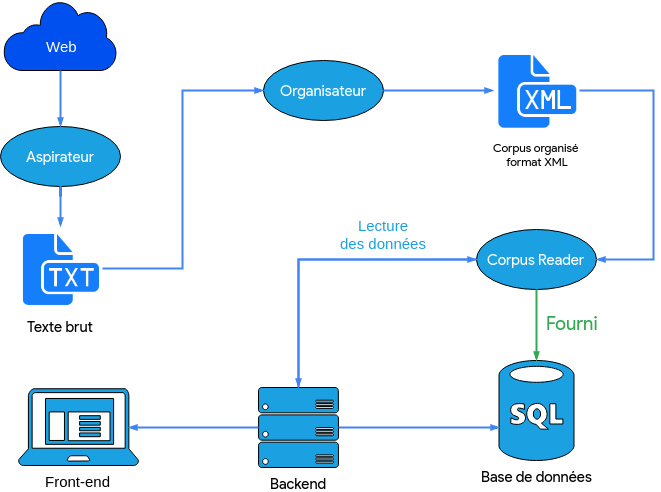
\includegraphics[scale=0.4]{images/app_schema.png}
			\caption{Schéma global du système}
			
		\end{figure}
		
	\section{Les modules du système}
		\paragraph{}
		Cette section se consacre à la description en détails des différentes modules du système, avec éventuellement des exemples d'utilisation de chacun.
		\subsection{Aspirateur de sites web}
			\paragraph{}
			Le module d'aspiration est composé de plusieurs petits scripts,
			le premier d'entre eux  \textbf{initializer.py} , son rôle est d'initialiser certaines
			variables globales (comme les dates de début/fin des périodes historiques de la langue arabe (\<العصر الجاهلي, عصر صدر الإسلام ... >), ou encore les chemins d'accès des différents fichiers récupérés et des fichiers xml produits.
			Il permet aussi la création dynamique d'une arborescence de répertoire où placer chaque fichier aspiré selon son époque, son genre, son type ...
			\par 
			Les autres scripts sont destiné à aspirer un type de document en particulier, nous pouvons citer les différents \textbf{"scrappeur"}\footnote{Terme anglais pour désigner un aspirateur de site web} utilisé : 
			\begin{itemize}
				\item \textbf{books\_scrape.py} Il a pour but d'aspirer le contenu du site \href{http://www.alwaraq.net/Core/index.jsp?option=1}{alwaraq.net}, qui est un recueil de livres arabes.
				
				\item \textbf{chi3r\_scrape.py} Son but est d'aspirer le contenu du site \href{https://www.aldiwan.net/}{aldiwan.net}, qui est une collection de poèmes arabes organisés par auteurs, périodes, pays ..., 
				
				\item \textbf{islamicbook\_scrape.py} Son but est d'aspirer le contenu du site \href{https://www.islamicbook.ws/}{islamicbook.ws}, qui est un 
				recueil d'ouvrages dédiés à l'islam.
				
				\item \textbf{news\_scrape.py} Son but est de télécharger les corpus déjà organisés depuis le site \href{http://aracorpus.e3rab.com/}{aracorpus.e3rab.com} qui est une banque de blogs rédigés en arabe.
%				
%				\item \textbf{shamela\_scrape.py} Il a pour but d'aspirer le contenu du site \href{http://shamela.ws/}{shamela.ws}, qui est un recueil de livres arabes déjà classifié en plusieurs sous catégories.
				
				\item \textbf{quran\_corpus\_builder.py} par respect pour les verset coraniques, nous avons décidé de télécharger un corpus déjà organisé sous format xml et certifié comme étant authentique par le groupe \textbf{Tanzil Project}(voir \href{http://tanzil.net/#19:3}{tanzil.net} ), puis nous l'avons ré-organisé en utilisant le script en une structure \textbf{XML} (que nous définirons plus bas).
				
			\end{itemize} 
			\par 
			Il a noté que tout ces scripts utilisent des fonctions d'organisation communes, pour placer chaque fichier acquis dans son répertoire adéquat dans l'arborescence créée par \textbf{initializer.py}, cela a pour but de faciliter l'accès ultérieur aux données bruts, pour les nettoyer et construire les corpus au format \textbf{XML}.
		\subsection{Organisateur de corpus}
			\paragraph{}
			Ce module est composé principalement d'un seul script qui effectue deux tâches, une fonction de nettoyage \textbf{"cleaner"}, et un constructeur de fichiers \textbf{\_cleanNotFound} pour générer le fichier \textbf{XML} associé a chaque texte brut extrait.
			Le format des fichiers XML que nous avons choisis est le suivant : 
			
			
			\begin{lstlisting}[language=XML]
			 	<root encoding="utf-8">
				 	<metadata>
					 	<book_name>`\< ألا حي بالبردين دارا ولا أرى >`</book_name>
					 	<era>Umayyad</era>
					 	<author>
						 	<name>`\< جرير >`</name>
						 	<birth>650</birth>
						 	<death>728</death>
						 	</author>
					 	<id>116</id>
					 	<type>`\<شعر>`</type>
					 	<size>66</size>
				 	</metadata>
					 	<doc>
						 	<sentence>`\<ألا حي بالبردين دارا ولا أرى>`</sentence>
						 	...
						 	<sentence>`\<كريما ولم تعلق عنانا يقيمها>`</sentence>
					 	</doc>
			 	</root>
			\end{lstlisting}
			
			\paragraph{Remarque : }
			Pour les textes coraniques, chaque \textbf{sura} (\<سورة>) sera représenté par un fichier \textbf{XML}, dont les balises 	\textbf{<sentence>} contiendront ses versets (\<آيات السورة>)
			
			\par
			Chaque document du corpus sera donc divisé en deux ensembles de balise, une partie méta-données contenant une variété d'information sur cet élément du corpus
			(Nom de l'auteur, période historique, id , type ...), puis une partie données, qui contiendra plusieurs phrases qui composent le document.
			\par 
			Après avoir construit l'arborescence, l'initialisation du système sera presque complète (il faudra remplir les tables de la base de donnés, nous verrons le schéma relationnel plus tard), il s'agira maintenant de passer la main au module suivant pour l'exploitation de ce corpus.
			
		\subsection{Corpus reader}
			\paragraph{}
			Ce module à joue le rôle d'une interface d'abstraction entre les fichiers XML et le serveur qui désire récupérer ces données,
			ce dernier devra instancier un objet de la classe \textbf{HistoricalCorpus}, cette classe hérite directement de la classe \textbf{nltk.corpus.XMLCorpusReader}, en redéfinissant les méthodes approprié, nous pourrons donc accéder au corpus et ses composants en 
			invoquant des méthodes comme : 
			\begin{itemize}
				
				\item 
				\begin{lstlisting}[language=python]
					def sents(fileid=None,start=None,end=None,era=None,category=None):\end{lstlisting} 
				Cette fonction retourne une liste de phrase du corpus tout entier, ou d'une portion selon les valeurs des paramètres qui lui sont passer (période,catégorie...).
				
				\item 
				\begin{lstlisting}[language=python]
					def tagged_sents(fileid=None,start=None,end=None,era=None,category=None):\end{lstlisting}
				Retourne une liste de phrases avec leurs étiquetages morpho-syntaxique.
				
				\item 
				\begin{lstlisting}[language=python]
				def lemma_sents(self,fileid=None,start=None,end=None,era=None,category=None):\end{lstlisting}
				Retourne une liste de phrases auxquelles une lemmatisation à été appliquée.
				
				
				\item 
				\begin{lstlisting}[language=python]
					def words(fileid=None,start=None,end=None,era=None,category=None):\end{lstlisting}
				Retourne une liste de tout les mots du corpus (ou d'une partie du corpus).
				
				\item 
				\begin{lstlisting}[language=python]
				def tagged_words(fileid=None,start=None,end=None,era=None,category=None):\end{lstlisting}
				Retourne une liste de tuples (mots,Étiquette-Morpho-Syntaxique) de tout les mots du corpus (ou d'une partie du corpus).
				
				\item 
				\begin{lstlisting}[language=python]
				def lemma_words(self, fileid=None,start=None,end=None,era=None,category=None):\end{lstlisting}
				Retourne une liste de de tout les lemmes (forme infléchie des mots) du corpus (ou d'une partie du corpus) 
				
				
			\end{itemize}
			\paragraph{}
			Le CorpusReader est invoqué principalement durant l'initialisation du serveur (avant l'utilisation de l'application), et cela pour garantir une utilisation plus aisée de l'application après déploiement. Il reste donc à voir comment le serveur remplit la base de données. 
		\subsection{Base de données}
			\paragraph{}
			Le but d'avoir cette base de données et principalement de stocker les différentes méta-données sur les documents du corpus, ainsi que les relations entres les contenus des documents, cela facilitera la tâche au serveur de ne considérer que le niveau le plus abstrait des données, et laisser la tâche de récupérer et manipuler ses données au CorpusReader.
			\par 
			Nous avons choisis le schéma relationnel suivant pour la base de données : 
			
			\begin{figure}[H]
				\centering
				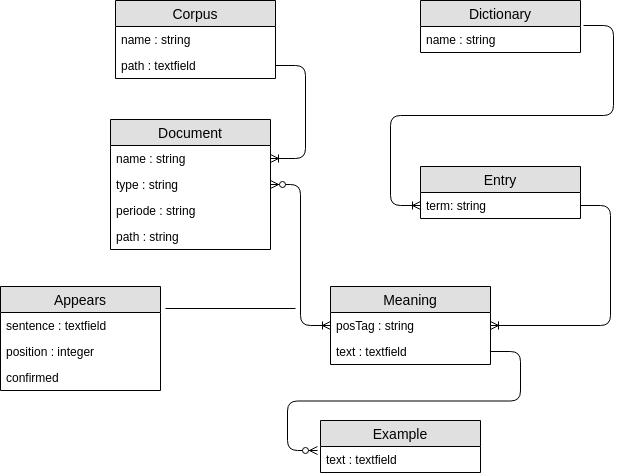
\includegraphics[width=0.65\linewidth]{images/db_schema.png}
				\caption{Schéma de la base de données }
			\end{figure}
		
			\par
			La table \textbf{Dictionary} est rempli avant la fin de la phase d'initialisation, nous avons pour cela utilisé les données provenant de deux sources : 
			\begin{itemize}
				\item \href{http://waqfeya.com/book.php?bid=6116}{\<المعجم الرائد >}
				\item \href{https://www.almaany.com/ar/dict/ar-ar/}{\<المعجم الجامع >}
				\item \href{http://waqfeya.com/book.php?bid=210}{\<المعجم الوسيط> }
			\end{itemize}
			Nous avons tout d'abord transformer les entrées du dictionnaire en un fichier \textbf{JSON} dont le format est le suivant : 
			\begin{lstlisting}[language=json,firstnumber=1]
			{
				"root"	 : 	{
							"postag-1"	:	[
								"def-1",
								...
							],
							
							...
							
							"postag-n"	:	[
							"def-1",
							...
							]
				},...
						
			}
			\end{lstlisting}
		\subsection{Application (Front-end et Back-end)}	
			\paragraph{Back-end :}
			C'est une application web qui expose une api REST-ful , elle est accessible a partir de certains \textbf{endpoints}\footnote{Emplacement dans le serveur renvoyant une réponse à une requête } qui seront exploités avec
			des requêtes \textbf{http}, l'avantage d'une telle architecture est qu'elle est 100\% interopérable 
			(elle ne dépends ni du système, ni des technologies ni du langage du serveur ou des clients).
			\paragraph{Front-end}
			le front-end utilise ces \textbf{endpoints} pour récupérer de la donnée et l'afficher à travers des requêtes lancée selon les besoins de l'utilisateur (en manipulant l'interface par exemple).
			On peut aussi développer une application mobile ou desktop de la même façon.   	
	\section{Déploiement des modules dans le cloud}
		\paragraph{}
		Nous avons choisi de déployer notre application suivant une architecture server-less dans le but de faciliter son utilisation, de la rendre publique et disponible à tout ceux qui voudraient la tester, donner un feedback ou proposer une amélioration en consultant le dépôt sur \href{https://github.com/mohammedi-haroune/arabic-historical-dictionary-frontend}{Github}
	\section{Conclusion}
		\paragraph{}
		Au terme de chapitre, nous avons donc fais le tour des principales composantes du système, sans trop rentrer dans les détails, nous introduirons les composantes non-citées dans le chapitre suivant lors de la présentation des fonctionnalités de l'application si besoin est.  
\chapter{Réalisation de l'application}
	\section{Introduction}
		\paragraph{}
		Durant ce chapitre, nous allons présenter l'aspect pratique de notre système, à savoir l'application qui lui est dédiée, nous commencerons par une description des outils utilisés, suivit d'une présentation de l'interface d'utilisation pour enfin introduire les fonctionnalités supplémentaire non-apparente dans cette dernière.  
	\section{Environnement de travail et outils utilisés}
		\subsection{Python}
			\begin{figure}[H]
				\centering
				
\includegraphics[width=0.25\linewidth]{images/python.png}
			\end{figure}
			\paragraph{}
			Python est un langage de programmation scripté très puissant, de par sa simplicité d'utilisation et de sa syntaxe
			très intuitive, il est aussi un des langages préférés des adeptes du TALN, pour la raison qu'un grand nombre de 
			bibliothèques y sont disponibles. Nous l'avons choisi principalement pour des traitement de TALN mais aussi dans la partie
			back-end  du système.
		\subsection{JavaScript}
			\begin{figure}[H]
				\centering
				
\includegraphics[width=0.25\linewidth]{images/js.png}
			\end{figure}
			\paragraph{}
			Très populaire chez les développeur web, JavaScript(JS) est un outil très puissant pour un développement rapide d'application web rapide, puissantes et élégantes.
		\subsection{NLTK}
			\paragraph{}
			 Natural Language Toolkit (NLTK) est un framework (ensemble de librairies) implémentant un grand nombre d'algorithmes et modèles du TALN, écrite en python elle sera donc parfaitement compatible avec notre back-end qui lui sera développé avec \textbf{DJANGO} (voir suite ).
		\subsection{VueJS}
			\paragraph{}
			\begin{figure}[H]
				\centering
				
\includegraphics[width=0.25\linewidth]{images/vjs.png}
			\end{figure}
			\paragraph{}
			Vue.js est un framework écrit en JavaScript pour le développement d'interface web, basé sur le principe de \textbf{components}, Vue donne au développeurs une grande liberté et flexibilité pour la création d'interface dynamiques
			et \textbf{reponsive}.
			
		\subsection{Django}
			\paragraph{}
			\begin{figure}[H]
				\centering
				
\includegraphics[width=0.25\linewidth]{images/django.png}
			\end{figure}
			\paragraph{}
			Django est un framework écrit en Python qui facilite le développement du back-end d'un site web, il s'occupe de gérer les couches basses de ce dernier (sessions, sécurité...)   et peut même générer une interface d'administration automatiquement. L’objectif  de Django est de proposer un développement plus efficace et plus rapide d'un site web dynamique tout en maintenant sa qualité.
		\subsection{PostgreSQL}
			\paragraph{}
			\begin{figure}[H]
				\centering
				
\includegraphics[width=0.25\linewidth]{images/postgresql.jpg}
			\end{figure}
			PostgreSQL est un système de gestion de base de données relationnelle et objet (SGBDRO). C'est un outil libre disponible selon les termes d'une licence de type BSD.
		
		\subsection{Google Cloud Platform}
			\paragraph{}
			\begin{figure}[H]
				\centering
				
\includegraphics[width=0.35\linewidth]{images/gcp.png}
			\end{figure}
		Google Cloud Platform est une plateforme de cloud computing fournie par Google, proposant un hébergement sur la même infrastructure que celle que Google utilise en interne pour des produits tels que son moteur de recherche1. Cloud Platform fournit aux développeurs des produits permettant de construire une gamme de programmes allant de simples sites web à des applications complexes.
	
	\section{Présentation de l'application}
		\subsection{Interface principale}
			\paragraph{}
			L'application se présente comme composé de trois partie, une barre d'outils en haut, un panneau d'onglet latéral permettant d'accéder au différentes section de l'application, et une zone d'affichage principale pour afficher le contenu de chaque section. 
		\subsection{Corpus}
			\paragraph{}
			Dans cette section, la main est donné à l'utilisateur pour uploader un nouveau corpus sur le serveur principal,  il suffit de donner un nom au corpus, une description pour faciliter son utilisation, et sélectionner les fichiers \textbf{XML} correspondant au corpus.
			
			%Upload new corpus into the server
		\subsection{Corpus Browser}
			\paragraph{}
			\begin{figure}[H]
				\centering
				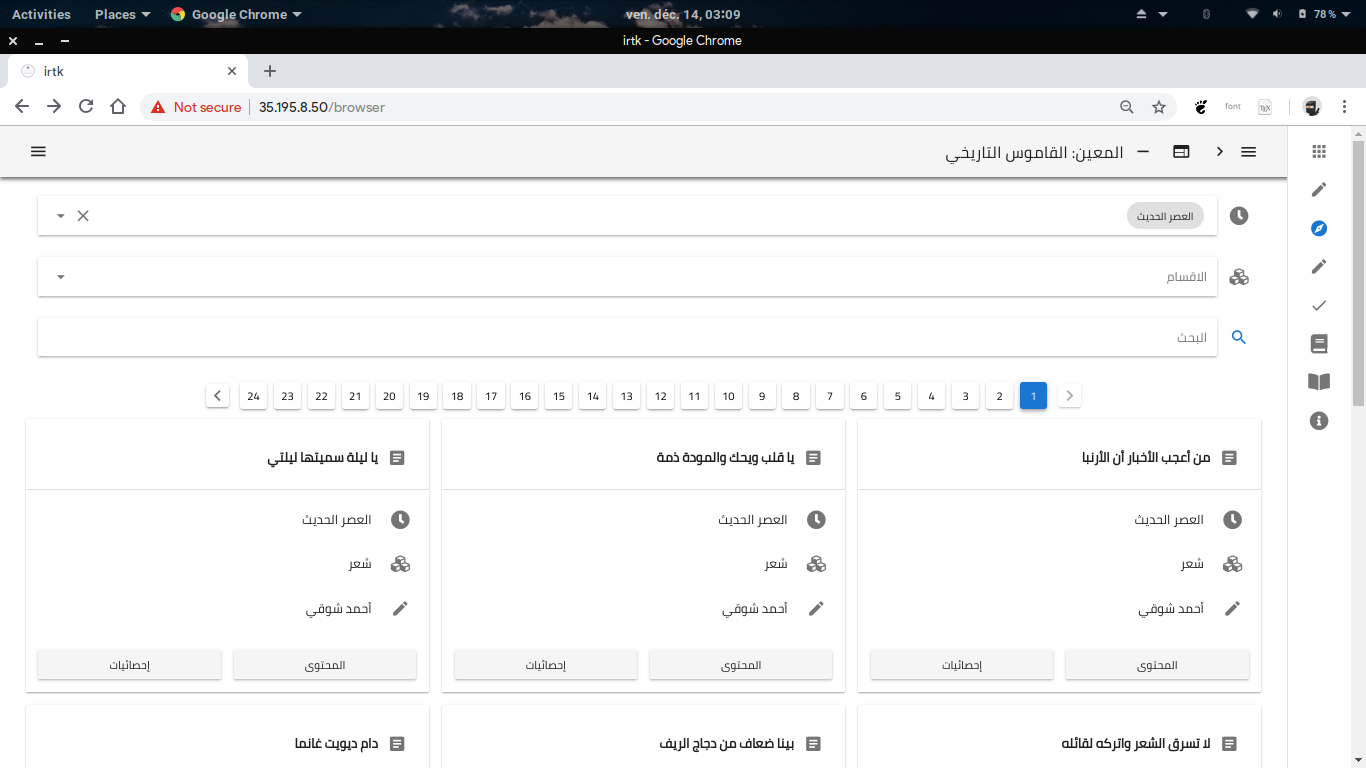
\includegraphics[width=0.8\linewidth]{images/app/corpusbrowser.png}
			\end{figure}
			Dans cette section, l'utilisateur pourra parcourir chaque composant du corpus, le choix lui est donné pour filtrer 
			sa recherche, que ce soit par période (\<الفترة الزمنية>), par section (\<قسم>) ou par mots clés, le résultats est une succession de pages dynamiquement ajoutées à la mémoire (grâce au corpus-reader), chaque page est composé de tuile contenant les informations relatives au documents pertinents selon le filtre de recherche.
			\par
			En cliquant sur le bouton \textbf{content} (\<المحتوى >), une nouvelle section est affichée, elle permet à l'utilisateur 
			de lire le fichier sélectionné. De plus s'il désire ajouter une nouvelle entrée au dictionnaire historique, il lui suffit de sélectionner la partie du texte qui l'intéresse , une liste déroulante s'affiche lui proposant d'ajouter un des mots précédemment sélectionnes au dictionnaire (nous verrons les détails de cette opération das la section suivante).
			
			%Explore the corporas
		\subsection{Add Entry}
			\paragraph{}
			\begin{figure}[H]
				\centering
				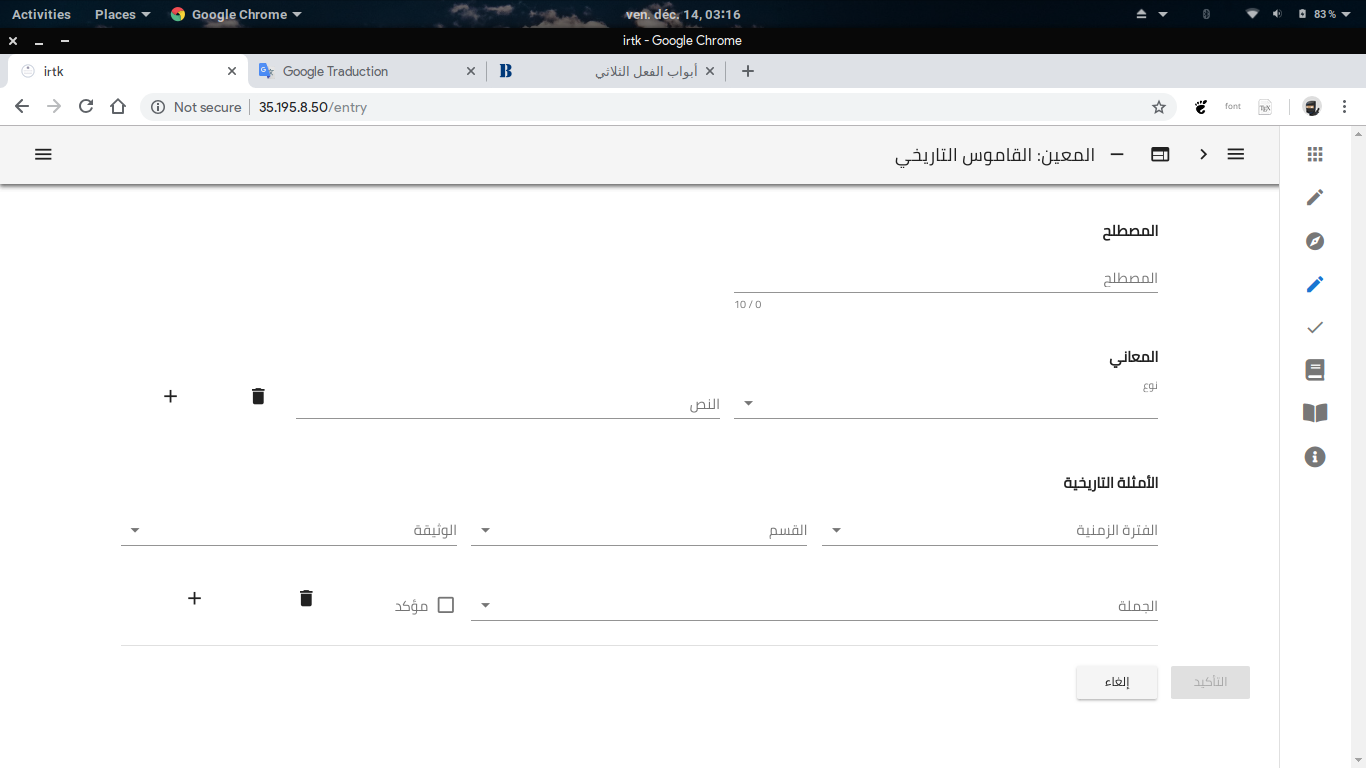
\includegraphics[width=0.8\linewidth]{images/app/addentry.png}
			\end{figure}
			Cette section donne la main au lexicographe pour ajouter une nouvelle entrée dans le dictionnaire historique, pour ce faire il faut entrer le terme à ajouter (\<المصطلح>), il faudra ensuite remplir un (ou plusieurs) champs selon le besoin
			de l'utilisateur : 
			\begin{itemize}
				\item Une liste de lignes réservées aux sens du termes à ajouter, il faudra fournir une étiquette morpho-syntaxique parmis une liste déroulante de choix possible (\<النوع>), suivit d'un extrait de texte où le terme apparaît (\<النص>).
				L'utilisateur pourra répéter ce processus autant de fois qu'il désire ajouter de sens au terme.
				
				\item Une liste de lignes réservées aux information chronologiques (\<الأمثلة التاريخية>), il faudra fournir la période historique (\<الفترة الزمنية>), la section visée (\<القسم>) , le document (\<الوثيقة>) puis finalement
				un exemple d'utilisation (\<الجملة>), un champ \textbf{confirmé} est à cocher pour valider la informations saisies, sinon l'ajout n'est pas autorisé.
			\end{itemize}
			%Add new entries into the historical dico
		\subsection{Dictionary}
			\paragraph{}
			\begin{figure}[H]
				\centering
				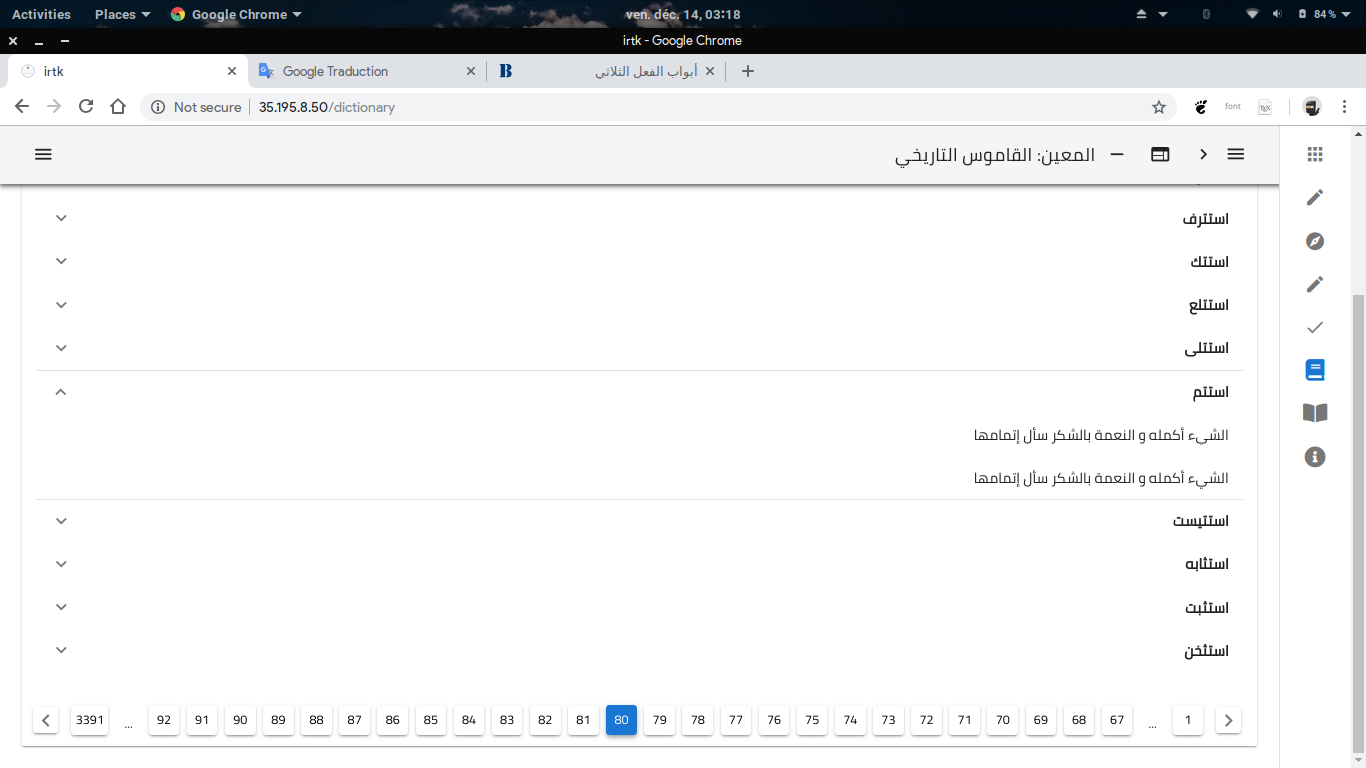
\includegraphics[width=0.8\linewidth]{images/app/allwords.png}
			\end{figure}
			Tout simplement cette section récupère tout les mots du dictionnaire classiques, et affiche les différents sens liés
			au mots auquel on s'intéresse.
%			All the words from the classical dico
			
		\subsection{Historical dictionary}
			\paragraph{}
			\begin{figure}[H]
				\centering
				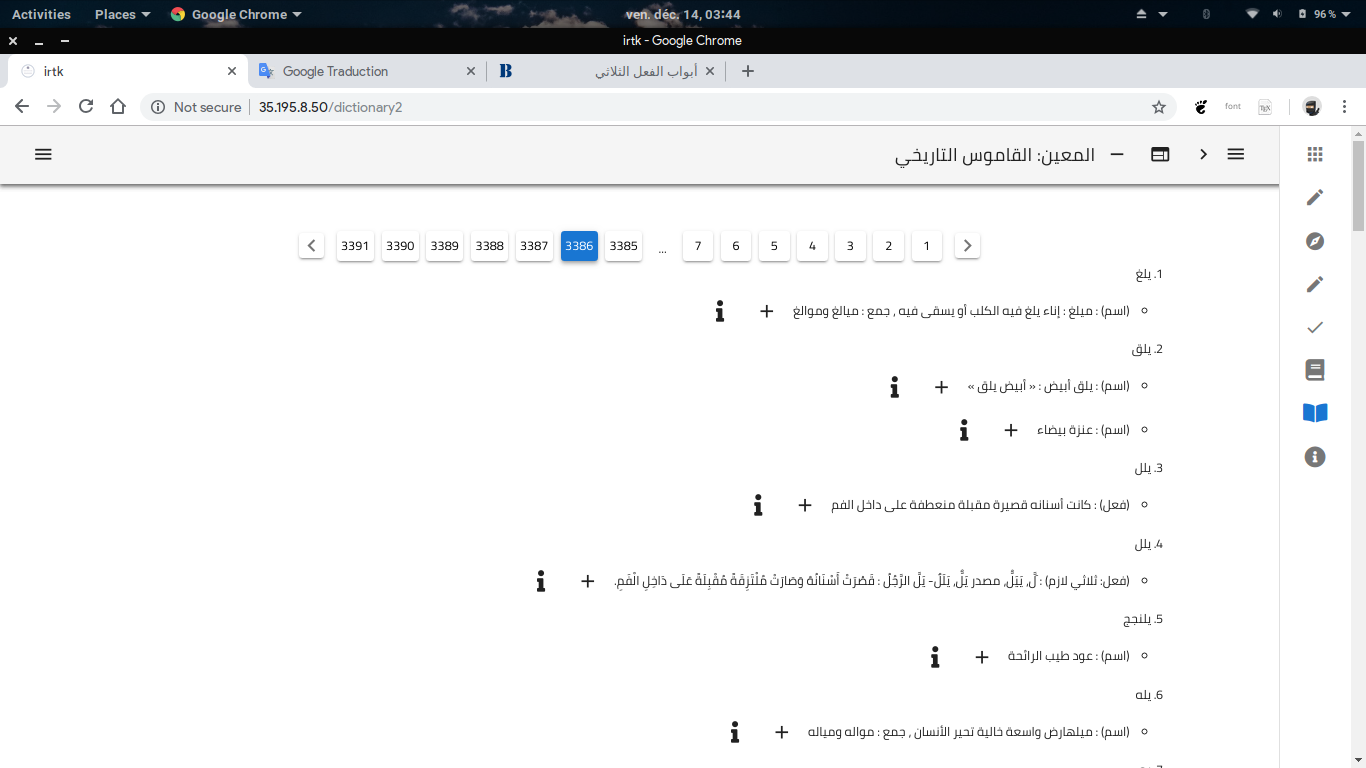
\includegraphics[width=0.8\linewidth]{images/app/histdico.png}
			\end{figure}
			Dans cette section, nous trouverons notre dictionnaire historique, organisé comme un dictionnaire classique avec des entrées(des mots) et leurs définitions, mais avec l'option de consulter les différentes utilisation du mot lors des siècles en cliquant sur un bouton, une timeline s'affiche en donnant un récapitulatif chronologique du mot : 
			
			\begin{figure}[H]
				\centering
				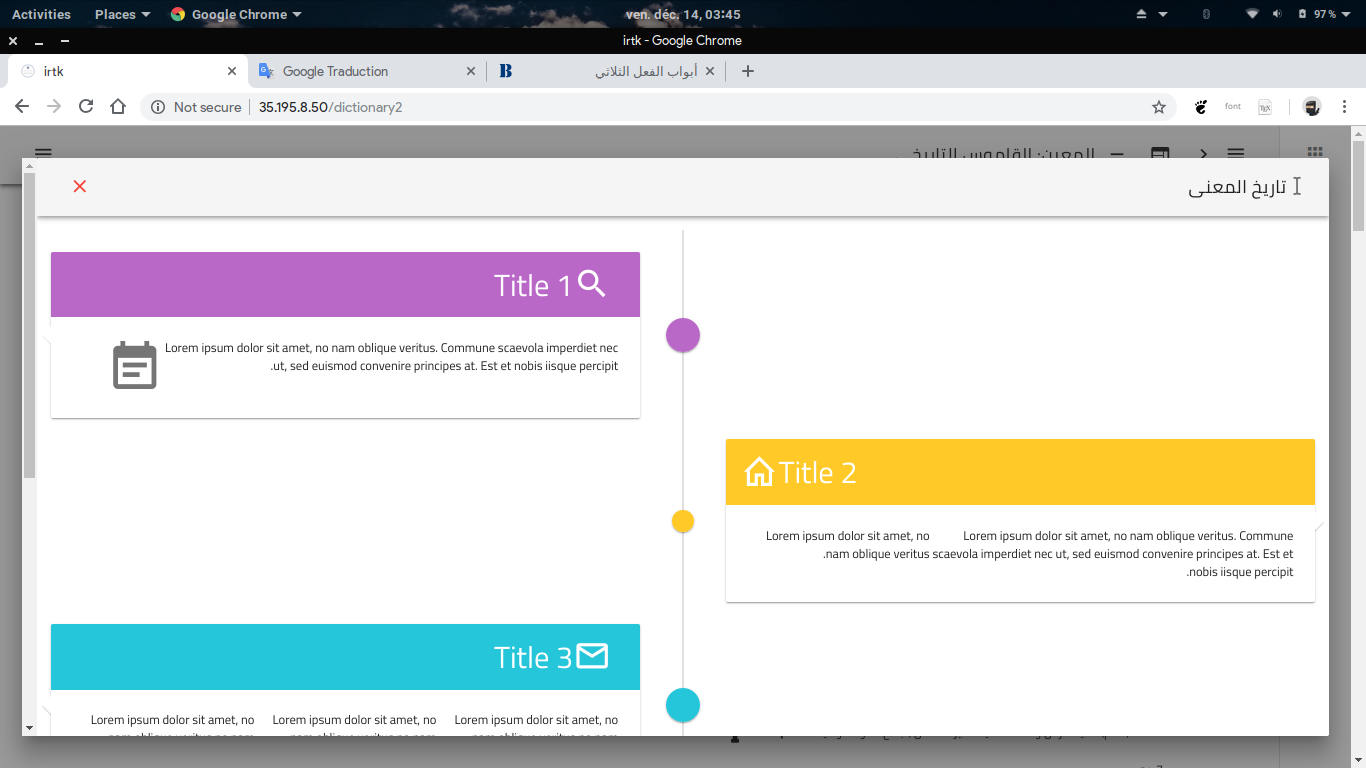
\includegraphics[width=0.8\linewidth]{images/app/histotimeline.png}
			\end{figure}
			\par
			L'option \textbf{+} permet de modifier cette entrée, elle renvoie à la section \textbf{add-entry} mais avec le champs \textbf{terme} déjà rempli avec le terme courant à modifier.
%		All the words from the historical dico
		\subsection{Graphs}
			\paragraph{}
			Display different statistics for some words
	\section{Fonctions supplémentaires}
	
	\section{Conclusion}


\chapter{Conclusion générale}
\section{Objectifs atteints}
\section{Limites du système}
\section{Perspectives futures}		

%mode auto is simple: 
%3andek f corpus method trodlek "apparition generator"  tmedelha list of words, and restrictions over corpus like category, era, fileid .. ou howa idir lemma sentences ta3 corpus and each time issib a word fhadouk lemmas irodlek the word m3a (fileid, sentence position fel file, word position fel sentence, a chunk of the sentence[optional]
\bibliographystyle{ieeetr}
\bibliography{ref}

\end{document}